\documentclass{article}
\usepackage[utf8]{inputenc}
\usepackage{fouriernc}
\usepackage[T1]{fontenc}
\usepackage{adjustbox}
\usepackage[margin=2cm]{geometry}
\usepackage{graphicx}
\usepackage{hyperref}
\usepackage{amsmath}
\usepackage{amsthm}
\usepackage{amssymb}
\usepackage{mathtools}
\hypersetup{colorlinks=true,linkcolor=blue,urlcolor=red}

\setlength{\parindent}{0pt}

\newtheorem{thm}{Theorem}[section]
\newtheorem*{thm*}{Theorem}
\newtheorem{prop}[thm]{Proposition}
\newtheorem*{prop*}{Proposition}
\newtheorem{defn}{Definition}[section]
\newtheorem*{defn*}{Definition}
\newtheorem{lem}[thm]{Lemma}
\newtheorem{cor}{Corollary}[thm]
\newtheorem{exa}{Example}
\newtheorem{exe}{Exercise}

\newcommand{\bb}[1]{\textbf{#1}}
\newcommand{\eps}{\varepsilon}
\newcommand{\N}{\mathbb{N}}
\newcommand{\Z}{\mathbb{Z}}
\newcommand{\R}{\mathbb{R}}
\newcommand{\pder}[2]{\frac{\partial #1}{\partial #2}}
\newcommand{\eval}[1]{\Big{|}_{#1}}
\newcommand{\scal}[2]{\langle #1 , #2 \rangle}
\newcommand{\del}{\partial}
\newcommand{\mc}{\mathcal}

\title{Graphs}
\author{}
\date{}
\begin{document}
    \maketitle
    \begin{section}{Graph Operators}
        
	\begin{defn}
            Let $\mc{G}$ be a graph where $\mc{V}$ are its vertexes and $\mc{E}$ are its edges, let $f,g : L^2(\mc{V})$ 
	    and $F,G \in L^2(\mc{E})$ be real valued functions, we define
	    $\scal{f}{g}_{L^2(\mc{V})} := \sum_\mc{V} a_i f_i g_i$, $a_i \in \R$ and
	    $\scal{F}{G}_{L^2(\mc{E})} := \sum_\mc{E} w_{ij} F_{ij} G_{ij}$, $w_{ij} \in \R$.
	\end{defn}
        
	\begin{defn}
	    \bb{Graph gradient and divergence}\\ 
	    Let $f \in L^2(\mc{V})$ and $F \in L^2(\mc{E})$ we define $grad : L^2(\mc{V}) \to L^2(\mc{E})$ and $div : L^2(\mc{E}) \to L^2(\mc{V})$,
	    such that $(gradf)_{ij}=f_i-f_j$ and $(divF)_i=\frac{1}{a_i}\sum_{j \in \mc{V} : (i,j) \in \mc{E}} w_{ij} F_{ij}$.
	\end{defn}

	\begin{prop}
	    Let $f \in L^2(\mc{V})$ and $F \in L^2(\mc{E}) : F_{ij}=-F_{ji}$ then $\scal{f}{divF}_{L^2(\mc{V})} = \scal{gradf}{F}_{L^2(\mc{E})}$,
	    i.e. $divF^\dag = grad$.
	\end{prop}
	\begin{proof}
	    $\sum_\mc{V} a_i f_i (divF)_i = \sum_{\mc{E}} w_{ij} F_{ij} (f_i-f_j) = \sum_{i \in \mc{V}}\sum_{j \in \mc{V} : (i,j) \in \mc{E}} w_{ij} F_{ij} f_i$
	    thus $a_i (divF)_i = \sum_{j \in \mc{V} : (i,j) \in \mc{E}} w_{ij} F_{ij}$.
	\end{proof}

	\begin{thm}
	    \bb{Fake Gauss theorem}\\
	    Let $F \in L^2(\mc{E}) : F_{ij}=-F_{ji}$, let $\mc{A} \subset \mc{V}$ then if $a_i = w_{ij} = 1$ we have
	    $\sum_{\mc{A}} (divF)_i = \sum_{\partial_+^0 \mc{A}} F_{ij}$.
	\end{thm}
	\begin{proof}
	    First of all we recall $\partial_+^0 \mc{A} = \{ (i,j) \in \mc{E}, i \in \mc{A}, j \in \mc{V \setminus A} \}$, then we see that
            $\sum_{\mc{A}} (divF)_i = \sum_{i \in \mc{A}}\sum_{j \in \mc{V} : (i,j) \in \mc{E}} F_{ij} =
	    \sum_{i \in \mc{A}}\sum_{j \in \mc{V \setminus A} : (i,j) \in \mc{E}} F_{ij} +
            \sum_{i \in \mc{A}}\sum_{j \in \mc{A} : (i,j) \in \mc{E}} F_{ij} = \sum_{\partial_+^0 \mc{A}} F_{ij} + \sum_{(i,j) \in \mc{A}^2} adj(\mc{A})_{ij} F_{ij}$
	    where since $adj(\mc{A})_{ij} = adj(\mc{A})_{ji}$ we have by renaming dummy indexes $adj(\mc{A})_{ij} F_{ij} = -adj(\mc{A})_{ij} F_{ij} = 0$.
        \end{proof}
	\begin{figure}[h]
	    \caption{Coboundary operator applied to A+B+C+D+E+F+U+V+W(green) and to A+B+C+D+E+F+U+V(green and red)}
	    \centering
            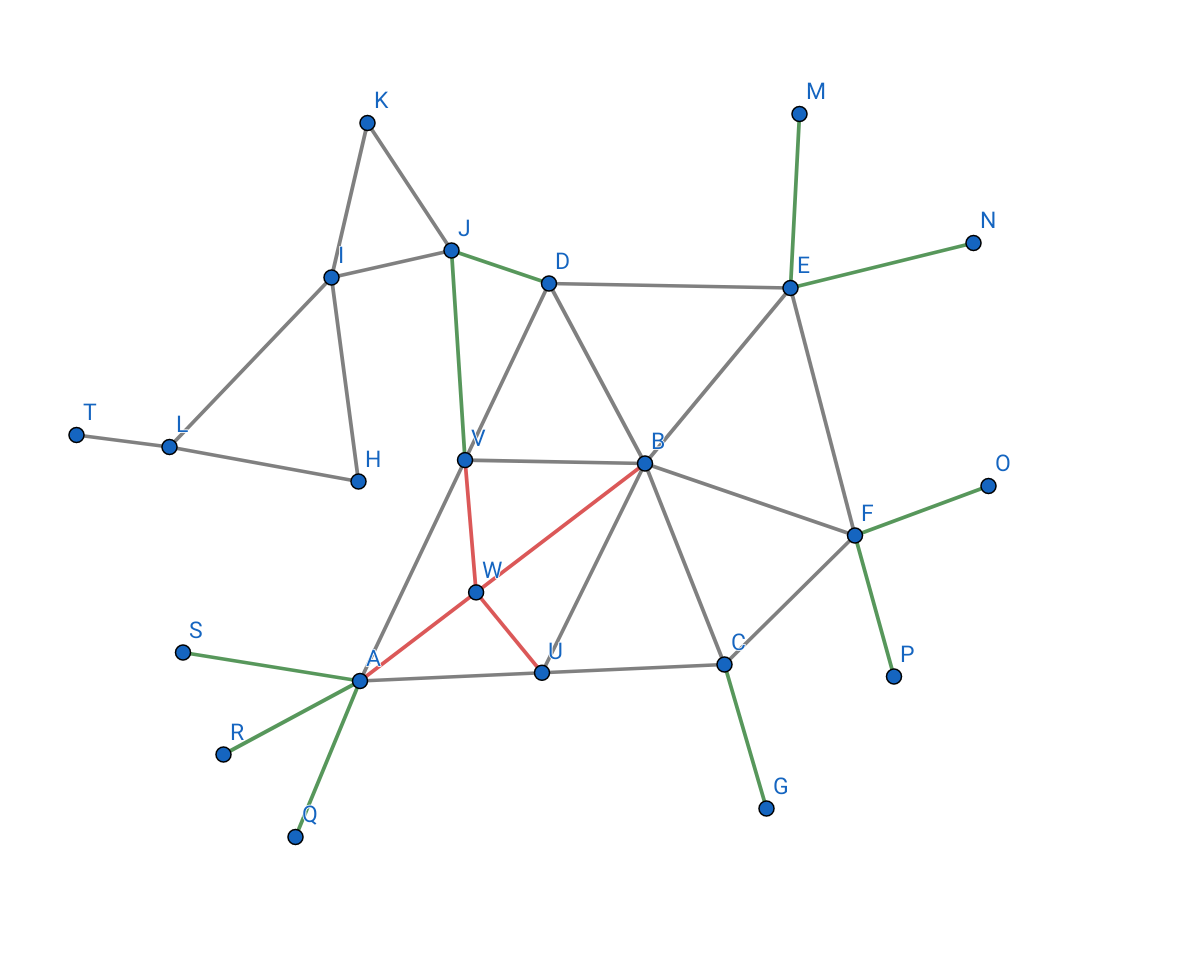
\includegraphics[scale = 0.3]{images/cobordo.jpg}
	\end{figure}
	
	\begin{prop}
	    The use of the coboundary operator makes sense only with antisimmetric functions on the edges, the antisimmetry of
	    those function is somehow related to the orientation of surfaces.
	\end{prop}
	\begin{proof}
	    $\sum_{\partial^0 \sum_{i \in \mc{A}} i}F_{ij} = \sum_{\sum_{i \in \mc{A}} \partial^0 i} F_{ij}$ if an edge
	    is in the coboundary of two different vertexes of $\mc{A}$ it will be count twice, that means zero times in $\Z_2$,
	    similarly for that same edge we would sum $F_{ij} + F_{ji} = 0$.
	\end{proof}

    
        \begin{defn}
	    \bb{Graph laplacian}\\
	    Let $f \in L^2(\mc{V})$ we have that $\scal{gradf}{gradf} = \scal{div(gradf)}{f} =: \scal{\Delta f}{f} = \scal{f}{\Delta f}$, where
	    $\Delta : L^2(\mc{V}) \to L^2(\mc{V})$ is the Laplacian.
	\end{defn}

	Possibili approfondimenti interessanti:\\
	(i)   Studio di equazioni differenziali sui grafi con gli operatori sopra definiti\\
	      -Equazione del Calore\\
	      $\frac{d(f_i)}{dt} = -c(\Delta f)_i$\\
	      -Equazione di Schr$\ddot{o}$dinger\\
	      $\frac{d(f_i)}{dt} = -c(\Delta f)_i + U_i f_i$\\
	      -Equazione di Navier-Stokes\\
	      -Equazione di continuità\\
	      -altre\\
	(ii)  Vincolare l'apprendimento di funzioni a divergenza nulla delle edge tramite $H^0$, eventuale applicazione a flussi incomprimibili\\
	(iii) Definire il rotore per 2-simplessi e fare l'analogo con $H_1$, eventuale applicazione a reti elettriche tridimensionali\\

    \end{section}
\end{document}
